\documentclass[12pt]{article} % Default font size is 12pt, it can be changed here
\usepackage{fontspec}
%Ligatures=TexOff disable the Tex specific ligatures which converst quotes into typographic quotes
\setmainfont{OpenSans}[Ligatures=TeXOff, Path=fonts/,Extension=.ttf, UprightFont=*-Regular, ItalicFont=*-Italic, BoldFont=*-Bold, BoldItalicFont=*-BoldItalic]
\usepackage{microtype}

%\usepackage{tabulary}
\usepackage{tabu} %span tables over multiple pages while still wrapping text inside cells
\usepackage{longtable} %needed by tabu package
\usepackage{geometry}
\geometry{a4paper, total={170mm,257mm}, left=20mm, top=20mm, }

\usepackage{graphicx} % Required for including pictures
\usepackage{tikz}
\usepackage{float} % Allows putting an [H] in \begin{figure} to specify the exact location of the figure
\usepackage{wrapfig} % Allows in-line images such as the example fish picture
\usepackage{lipsum} % Used for inserting dummy 'Lorem ipsum' text into the template

\newcommand{\sectionbreak}{\clearpage}

\graphicspath{{../graphics/}} % Specifies the directory where pictures are stored 

\usepackage{tcolorbox}
\tcbuselibrary{skins}

\usepackage{listings} % Code listings
\usepackage{color}

\definecolor{dkgreen}{rgb}{0,.6,0}
\definecolor{dkblue}{rgb}{0,0,.6}
\definecolor{dkyellow}{cmyk}{0,0,.8,.3}
\definecolor{codegreen}{rgb}{0,0.6,0}
\definecolor{codegray}{rgb}{0.5,0.5,0.5}
\definecolor{codepurple}{rgb}{0.58,0,0.82}
\definecolor{backcolour}{rgb}{0.95,0.95,0.92}

%\lstset{
%  language        = php,
%  basicstyle      = \scriptsize\ttfamily,
%  keywordstyle    = \color{dkblue},
%  stringstyle     = \color{red},
%  identifierstyle = \color{dkgreen},
%  commentstyle    = \color{gray},
%  emph            =[1]{php},
%  emphstyle       =[1]\color{black},
%  emph            =[2]{if,and,or,else},
%  emphstyle       =[2]\color{dkyellow}}

\lstdefinestyle{phpStyle}{
    language=PHP,
    basicstyle=\scriptsize\ttfamily,
    commentstyle=\color{codegreen},
    keywordstyle=\color{blue},
    numberstyle=\tiny\color{codegray},
    stringstyle=\color{codepurple},
    backgroundcolor=\color{backcolour},
    breakatwhitespace=false,
    breaklines=true,
    captionpos=b,
    keepspaces=true,
    showspaces=false,
    showstringspaces=false,
    showlines=true,
    showtabs=false,
    tabsize=4
}

\setlength{\parindent}{0pt} % removes the default indentation of first lines
\setlength{\tabcolsep}{12pt}

\NewEnviron{squeeze}{\scalebox{.9}[1.0]{\BODY}}
\NewEnviron{squeezealot}{\scalebox{.8}[1.0]{\BODY}}

\newenvironment{mono}{\ttfamily}{\par}
\newenvironment{keyword}{\leavevmode\color{magenta}}{}
\newenvironment{keywordpurple}{\leavevmode\color{purple}}{}
\newenvironment{examplecomment}{\leavevmode\color{magenta!60!white}}{}
\newenvironment{code}{\begin{mdframed}[linewidth=4pt, linecolor=blue!40, topline=false, bottomline=false, rightline=false, backgroundcolor=blue!10]
                          \begin{mono}}{\end{mono}
\end{mdframed}}

\newenvironment{properties}
{
    \footnotesize\renewcommand{\arraystretch}{1.30}
    \renewcommand{\tabcolsep}{0pt}
    \begin{longtable}{>{\begin{keyword}}p{3.1cm}<{\end{keyword}}p{13.9cm}}
        \hline
        }
        {
        \hline
    \end{longtable}\vspace{5mm}
}

\newenvironment{parameters}
{
    \footnotesize\renewcommand{\arraystretch}{1.30}
    \renewcommand{\tabcolsep}{0pt}
    \begin{longtable}{>{\begin{keyword}}p{3cm}<{\end{keyword}}>{\begin{em}}p{1.5cm}<{\end{em}}p{12.5cm}}
        \hline
        }
        {
        \hline
    \end{longtable}\scriptsize\vspace{-5mm}*mandatory parameters\vspace{5mm}
}

\newtcolorbox{exampleResultBox}[2][]{
    skin=bicolor,colback=magenta!10!white,
    fonttitle=\bfseries,
    colbacktitle=magenta,
    bottomtitle=2mm,
    toptitle=2mm,
    colbacklower=black!10!white,
    title=#2,#1,
    boxrule=0mm,
    middle=0mm,
    boxsep=0mm,
    left=5mm,
    right=5mm,
    bottom=5mm,
    top=5mm,
    after upper={\hyphenpenalty=10000\raggedright\vskip 5mm\null},
    subtitle style={colback=black,left=5mm,right=5mm,bottom=2mm,top=2mm}
}

\newtcolorbox{exampleBox}[2][]{
    colback=magenta!10!white,
    fonttitle=\bfseries,
    colbacktitle=magenta,
    boxrule=0mm,
    title=#2,#1
}

\newtcolorbox{resultBox}[2][]{
    colback=black!20!white,
    fonttitle=\bfseries,
    colbacktitle=black,
    boxrule=0mm,
    title=#2,#1
}

\newtcolorbox{advancedBox}[2][]{
    colback=purple!10!white,
    fonttitle=\bfseries,
    colbacktitle=purple,
    boxrule=0mm,
    title=#2,#1
}


\setlength{\parskip}{0.5em}

\DeclareTextFontCommand{\kw}{\keyword}
\DeclareTextFontCommand{\kwp}{\keywordpurple}

\begin{document}
    \small

%----------------------------------------------------------------------------------------
%	TITLE PAGE
%----------------------------------------------------------------------------------------

    \begin{titlepage}

        \newcommand{\HRule}{\rule{\linewidth}{0.5mm}} % Defines a new command for the horizontal lines, change thickness here

        \center % Center everything on the page

        \begin{tikzpicture}[remember picture,overlay]
            \node[anchor=north west,inner sep=1cm] at (current page.north west){
\includegraphics[width=3cm]{logos/UniLogo}};
        \end{tikzpicture}

        \begin{tikzpicture}[remember picture,overlay]
            \node[anchor=north east,inner sep=1cm] at (current page.north east){
\includegraphics[width=6cm]{logos/LUCET}};
        \end{tikzpicture}\\[6cm]

        \textsc{\large OASYS v3.6}\\[0.5cm] % Software version this document applies to

        \HRule \\[0.4cm]
        { \huge \bfseries API reference}\\[0.4cm] % Title of document
        \HRule \\[1.5cm]

        \large
        \textit{Author:} Eric J. FRANCOIS % Your name
        \begin{tikzpicture}[remember picture,overlay]
            \node[anchor=south,inner sep=2cm] at (current page.south){\large \today};
        \end{tikzpicture}

    \end{titlepage}

    \newpage


    \section{general information}\label{sec:general-information}

    OASYS provides a number of APIs that allow external sources to fetch data from OASYS, trigger OASYS to show the preview of an item or even to inject information (e.g.\ creation of test takers controlled from an outside source).

    While some APIs, like previewing an item, require to work with a permanent link that can be sent via e-mail for review, the APIs that actually modify the data inside OASYS (e.g.\ creation of back end users) require a higher security, to make sure a url including its parameteres can only be executed once and only one specific instance of OASYS\@.

    For this reason there are two different types of APIs: the high security and the low security ones.
    Both APIs have one thing in common: Before they can be used, an API key needs to be created in the database table \kw{apiKeys}, for the application that wants to use OASYS. This ensures that only known sources can use a specific instance of OASYS. The api key is linked to one specific API, so that an application does not automatically get permission to use every available API. Each permission needs to be given by a new entry in the \kw{apiKeys} table.\\

    The API URL is always:\\
    \ttfamily http(s)://<baseurl of OASYS>/api/<name of API to use>\\

    \sffamily For example:\\
    \ttfamily https://demo.oasys.lu/api/createUser/

    \sffamily


    \section{high security APIs}\label{sec:high-security-apis}

    In addition to the API key, a high security API requires a secret to be specified in the \kw{apiKeys} table.
    This secret needs to be known to the application using the API. The secret will never be transmitted.

    \begin{center}
        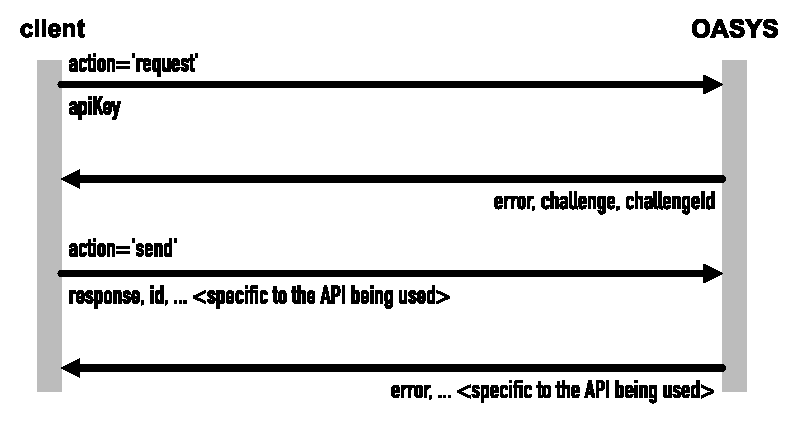
\includegraphics[width=12cm]{OASYS_api_chart_1}
    \end{center}

    As seen in the chart, there are a few steps to use this kind of API:

    \begin{enumerate}
        \item The client needs to request the use of the API by transmitting its API key.
        The following GET or POST parameters need to be sent:
        \begin{itemize}
            \item \kw{action} = 'request'
            \item \kw{key} = <the API key>
        \end{itemize}
        \item The API now saves the request in the \kw{apiRequests} table with the current timestamp.
        The request will only be valid for the next minute.
        OASYS sends back a JSON object that will contain a key called \kw{error} with a string if something went wrong (e.g.\ unknown API key), or if everything succeeded, it will contain the two keys \kw{challenge} and \kw{challengeId}.\\\\
        The \kw{challenge} key will contain a string necessary to create a valid response and the \kw{challengeId} key contains an integer which identifies the request in the \kw{apiRequests} table.
        \item The client will now calculate a proper response by concatenating the secret and the challenge and then hashing the string with an algorithm supported by PHP (by default BCRYPT since PHP 5.5).
        Then it will contact the API again—within 1 minute—and transmit the following GET or POST parameters:
        \begin{itemize}
            \item \kw{action} = 'send'
            \item \kw{response} = <the hashed response>
            \item \kw{id} = <the request id that was transmitted by the client>
            \item \ldots any other information necessary for the particular API being used
        \end{itemize}
        \item The API will now check if the request still exists and if the response to the challenge is valid.
        Then it will delete the request from the table, so that it cannot be used again later with the exact same parameters.\\\\
        If everything checks out, the rest of the parameters are being checked by the API then it returns another JSON object that may contain an \kw{error} or if everything succeeded the expected data (check specific APIs for the exact data to expect).

    \end{enumerate}


    \section{low security APIs}\label{sec:low-security-apis}
    Currently there are no low security APIs yet in OASYS


    \section{specific API details}\label{sec:specific-api-details}

    \subsection{createUser}\label{subsec:createuser}

    \textbf{API type:} high security

    This API allows to create a backend user (e.g.\ to give demo access to the editor of OASYS).
    The client needs to send a login for the user and the name of an existing usergroup which the user should be added to.
    Optionally a password can be specified for the new user.
    If omitted, a password will be generated randomly and sent back.\\

    \begin{minipage}{\textwidth}
        \textbf{input parameters:}
        \begin{parameters}
            username *  & string & the login to be used—this needs to be no longer than 32 characters and may contain letters, numbers, understores, hyphens and periods. \\
            usergroup * & string & the name of the group to add the user to—this needs to exist already, otherwise the creation will fail.                                \\
            password    & string & the password to be used—this must not exceed 32 characters                                                                             \\
            email       & string & the e-mail address of the user to be created, this is optional and will be ignored if it's not a valid e-mail address. \\
        \end{parameters}
    \end{minipage}

    \begin{minipage}{\textwidth}
        \textbf{returned data:}
        \begin{properties}
            error     & error message if something went wrong                                         \\
            username  & the login that was requested                                                  \\
            usergroup & the usergroup that was sent to the API                                        \\
            password  & the password that was requested, respectively the randomly generated password \\
            email     & the e-mail address that was sent to the API, respectively an empty string if it was not valid \\
        \end{properties}
    \end{minipage}

    \subsection{createTestTaker}\label{subsec:createtesttaker}

    \textbf{API type:} high security

    This API allows the creation of a list of test takers (with login, meta data, password, password tag, one or more tests to be linked) in an existing folder.
    Everything is optional except for the login and the test(s) to be linked.
    All parameters other than the logins can either be passed globally to be applied to all test takers (e.g.\ a common password for the whole class) or individually for each test taker.
    If both an individual parameter and a global one is set, the individual one is being used.

    \begin{minipage}{\textwidth}
        \textbf{input parameters:}
        \begin{parameters}
            testTakers * & JSON    & array of test takers to create, see below for details on this array                                                           \\
            password     & string  & a global password to be used for all test takers                                                                              \\
            testIds      & JSON    & array of test ids to be linked with every login—these are the internal ids of tests and they must exist in order to be linked \\
            folderId     & integer & the id of the folder all the test takers are to be created in                                                                 \\
            metaData     & JSON    & array of key-value pairs of meta data to be added globally to every test taker (e.g.\ name of the school)                     \\
            tag          & string  & a tag to be applied to all passwords created                                                                                  \\
        \end{parameters}
    \end{minipage}

    \begin{minipage}{\textwidth}
        \textbf{keys in each test taker in the array:}
        \begin{parameters}
            login *   & string  & the actual login to be entered                                                                                               \\
            password  & string  & a password to used for this test taker—if omitted, a random password will be created and returned                            \\
            testIds * & array   & array of test ids to be linked with this login—these are the internal ids of tests and they must exist in order to be linked \\
            folderId  & integer & the id of the folder the test taker is to be created in                                                                      \\
            metaData  & array   & array of key-value pairs to be added to the test taker                                                                       \\
            tag       & string  & a tag to be applied to the current password                                                                                  \\
        \end{parameters}
    \end{minipage}

    \textbf{Attention:} While the arrays \kw{testIds} and \kw{metaData} need to be JSON encoded when sent as a global parameter, they must not be JSON encoded when part of a test taker as the \kw{testTakers} array already is JSON encoded—there is no use encoding it twice. \\\\

    \begin{minipage}{\textwidth}
        \textbf{returned data:}
        \begin{properties}
            error      & error message if something went wrong                                                                                                                                                                                                                    \\
            testTakers & the same array that was sent to the API with an additional error field with a message if anything did not go according to plan.                                                                                                                          \\
            & If no password was specified it will also contain the password (either a randomly generated one, or a previously existing one from the database)                                                                                                         \\
            & There is also an extra field called \kw{state} which will be \textbf{true} if the current credentials are available for login and \textbf{false} if the credentials already existed and have been used, so that no further login is possible any longer. \\
        \end{properties}
    \end{minipage}

    \begin{minipage}{\textwidth}
        Depending on which parameters are sent, this API adopts a different behaviour: \\\\
        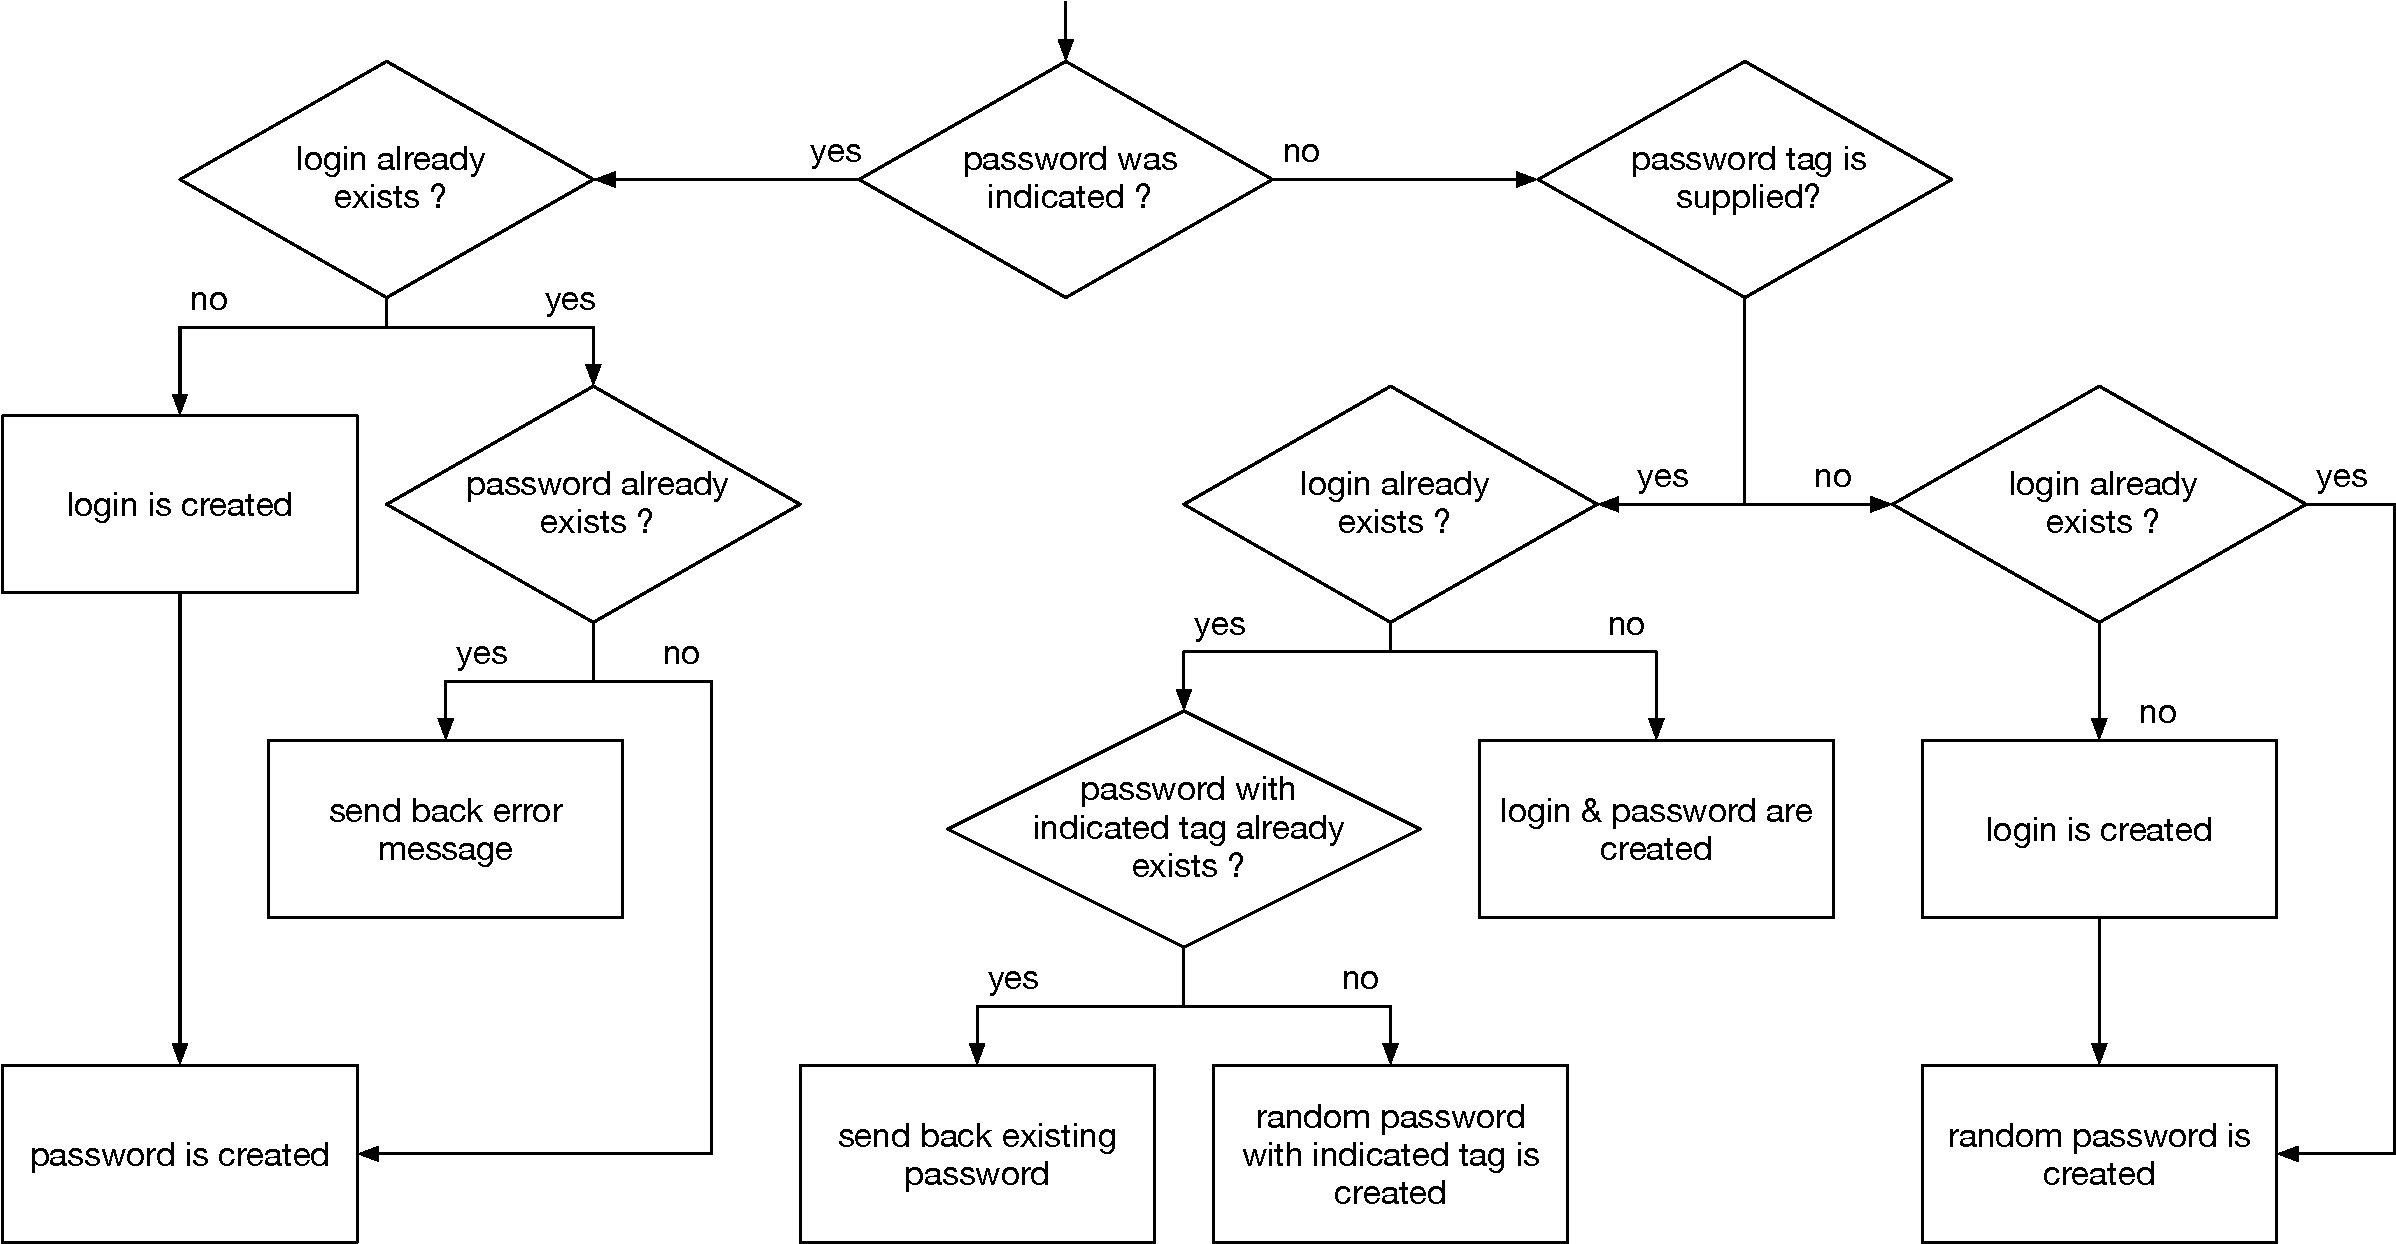
\includegraphics[width=\textwidth]{OASYS_api_createTestTaker_1}

    \end{minipage}

    \subsection{getProgress}\label{subsec:getprogress}

    \textbf{API type:} high security

    This API allows checking the progress of a specific login and test combination.
    If the test taker has filled in the same test multiple times (by the means of different passwords), the latest password will be taken (the password with the highest auto increment id).
    If more passwords exist, linking the test taker to the exact same test, it is possible to distinguish the passwords by the use of tags, which can optionally be indicated here as well.

    \begin{minipage}{\textwidth}
        \textbf{input parameters:}
        \begin{parameters}
            login *  & string  & the login for which the progress is requested                                                         \\
            testId * & integer & the internal id of the test for which the progress is requested                                       \\
            tag      & string  & the tag of the password we are looking for—if the tag is null or not sent at all, it will be ignored. \\
        \end{parameters}
    \end{minipage}

    \begin{minipage}{\textwidth}
        \textbf{returned data:}
        \begin{properties}
            error      & error message if the request failed—false if everything went smoothly \\
            status $\rightarrow$ started & 0 if test taker never logged in to this test;
            1 if there has been activity \\
            status $\rightarrow$ finished & 0 if the test taker can still log in and change data;
            1 if the test has been finalised \\      & (e.g.\ answers were submitted respectively the time ran out)                                \\
            total    & the total count of fields in this test                  \\
            answers & the count of fields to which the test taker answered                                 \\
            percentage & percentage of fields that were filled                                 \\
        \end{properties}
    \end{minipage}


    \textbf{Attention:} Beware of tests with conditional branching.
    There is no way to predict exactly which pages were hidden from the test taker at this point, so the total number of fields may be higher than those that were really available to the test taker. \\\\

    \subsection{getTestProgress}\label{subsec:gettestprogress}

    \textbf{API type:} high security

    This API allows checking the progress of a specific test for all logins that have been active in this test.
    If a test taker has filled in the same test multiple times (by the means of different passwords), the latest activity will be taken (based on the last login timestamp).
    Furthermore it is possible to define two types of filters: you can define to only get the progress of passwords with a specific tag and you can define a cutoff date in order to ignore any data collected before that date.

    \begin{minipage}{\textwidth}
        \textbf{input parameters:}
        \begin{parameters}
            testId *                         & integer & the internal id of the test for which the progress is requested                                  \\
            filters                          & JSON    & an array which can define additional filters—the keys 'tags' and 'cutoffDate' are supported here \\
            filters $\rightarrow$ tags       & array   & list of strings that are considered acceptable password tags                                     \\
            filters $\rightarrow$ cutoffDate & string  & a date in the form YYYY-MM-DD in order to ignore any data gathered before this date.             \\
        \end{parameters}
    \end{minipage}

    \begin{minipage}{\textwidth}
        \textbf{returned data:}
        \begin{properties}
            error    & error message if the request failed—false if everything went smoothly \\
            activity & array of logins and their progress data, see below for details        \\
            total    & the total count of fields the test contains                           \\
        \end{properties}
    \end{minipage}

    \begin{minipage}{\textwidth}
        \textbf{returned activity data (in activity $\rightarrow$ <login>):}
        \begin{properties}
            login      & login string (duplicate of the key)                  \\
            tag        & password tag, if any                                 \\
            started    & 0 if the test taker never logged in to this test, 1 if there has been activity \\
            finished & 0 if the test taker can still log in and change data;
            1 if the test has been finalised \\    & (e.g.\ answers were submitted respectively the time ran out) \\
            answers & the count of fields to which the test taker answered      \\
            lastAnswer & timestamp of the last answer given in this test                \\
            percentage & percentage of fields that were filled                \\
        \end{properties}
    \end{minipage}


    \textbf{Attention:} Beware of tests with conditional branching.
    There is no way to predict exactly which pages were hidden from the test taker at this point, so the total number of fields may be higher than those that were really available to the test taker. \\\\

    \subsection{editTestTaker}\label{subsec:edittesttaker}

    \textbf{API type:} high security

    This API allows making modifications to the activity of a test taker, resp.\ to the test taker itself. It can change the time left for a test, reset the activity entirely, set current page of a test taker or rename the login of a test taker.

    \begin{minipage}{\textwidth}
        \textbf{input parameters:}
        \begin{parameters}
            login *  & string  & the login to be edited                                                                                                                                                                 \\
            testId * & integer & the internal id of the test for which activity is to be edited                                                                                                                         \\
            tag      & string  & the tag of the password we are looking for—if the tag is null or not sent at all, it will be ignored.                                                                                  \\
            tasks *  & JSON    & array of tasks to be executed, whereas each task consists on an array with the property \kw{task} describing the action to be done and if necessary a property \kw{value} (see below for details) \\
        \end{parameters}
    \end{minipage}

    \begin{minipage}{\textwidth}
        \textbf{defined keywords for the 'task' property:}
        \begin{properties}
            resetActivity  & deletes all activity for login and testId combination, no value required                                             \\
            setTimeLeft    & change the time left, \kw{value} property must be an integer (time in seconds, or -1 for no limit)                        \\
            setCurrentPage & set the page to be shown to the test taker after next login, \kw{value} property must be an integer (start counting at 0) \\
            changeLogin    & rename the login, \kw{value} property must be a string with the new name                                                  \\
        \end{properties}
    \end{minipage}

    \begin{minipage}{\textwidth}
        \textbf{returned data:}
        \begin{properties}
            error & error message if the request failed—false if everything went smoothly\\
        \end{properties}
    \end{minipage}

    \begin{minipage}{\textwidth}
        \textbf{notes:}
        \begin{itemize}
            \item Even though renaming a login does not require a testId, it is still required as a sanity check. If a login is indicated with a testId that does not exist, we have to assume that the request is a mistake (or worse, an attack).
            \item When using \kw{setTimeLeft} with value -1 this cannot override a time limit set in the test. In this case the test taker will get the maximum allowed time.
            \item If \kw{setTimeLeft} is used with a value higher than 0, it is possible to give more time than the test allows. This is useful if a test taker has to be given extra time due to a handicap.
            \item Renaming a login will not allow to rename it to an already existing login. If a login is specified that exists, the request will fail with an error message.
            \item The \kw{setCurrentPage} task should be used in combination with \kw{setTimeLeft} when reopening an already submitted test. If the time left was 0 and is now set to -1 (or any positive value), the test taker would normally see the last page with the submit button when logging in again. Here it is advisable to set the current page to 0, so that the test taker will see the first page again by default.
        \end{itemize}
    \end{minipage}

    \pagebreak

    \section{PHP example of using a high security API}\label{sec:example-high-security}

    \begin{lstlisting}[style=phpStyle, label={lst:example_01}]

	<?php
	$protocol = "https://";
	$url = "demo.oasys.lu/oasys/api/getTestProgress/";

	$apiKey = 'getTestProgressDemo';
	$secret = 'demo';
	$testId = 42;
	$filters['tags'] = ['demotag'];
	$filters['cutoffDate'] = '2023-05-01';

	$data = file_get_contents($protocol . $url . "?action=request&key=$apiKey");
	$data = json_decode($data);

	if ($data->error) {
		print_r($data);
		die();
	}

	$response = password_hash($secret . $data->challenge, PASSWORD_DEFAULT);
	$id = $data->challengeId;

	$postData = http_build_query([
		'action' => 'send',
		'response' => $response,
		'id' => $id,
		'testId' => $testId,
		'filters' => json_encode($filters)
	]);

	$opts = [
		'http' => [
			'method' => 'POST',
			'content' => $postData,
			'ignore_errors' => true,
			'header' => 'Content-type: application/x-www-form-urlencoded',
			'ssl' => [
				'verify_peer' => false,
				'verify_peer_name' => false
			]
		]
	];

	$context = stream_context_create($opts);
	$raw = file_get_contents($protocol.$url, false, $context);

	$data = json_decode($raw, true);

	if (json_last_error() != JSON_ERROR_NONE) {
		echo "<p>Error decoding answer (JSON error " . json_last_error() . ")!</p>";
		echo "<pre>$raw</pre>";
		die();
	}

	echo "<pre>";
	print_r($data);
	echo "</pre>";

    \end{lstlisting}

\end{document}

